\section {Глава 2. Создание игры и написание скриптов}
\subsection{Изучение аналогов.}
Конечно для разработки видеоигры и ее основных механик я
ориентировался на проекты схожие с моим. В итоге я выбрал 5 проектов
наиболее схожим с моим, а именно: “ Dragon Age :Origins”, “ Harry Potter”,
“Mages of Mystralia”, “ Atom RPG”, “ Tales of Arise”
Таблица 1. Обзор аналогов \newline
\begin {center}
\begin{tabular}{ | m{6em} | m{3cm}| m{5cm} | m{3cm} | m{3cm} | } 
 \hline
Название & Движок & Цель & Управление & Жанр\\
 \hline
 Dragon Age:Origins &  ECLIPSE &путешествие
мага-воина с
целью
уничтожения
зла &мышь & фэнтези, вид
сверху, экшн,
RPG\\
\hline
 Harry Potter &Unreal Engine 4 &путешествие
ученика у
волшебной
школе с
целью
уничтожения
зла и
изучению
новых
заклинаний& мышь и
клавиатура&фэнтези, вид
сверху, экшн\\
\hline 
Mages of Mystralia & unity & победить
могучих
существ и
пройти
квесты, с
помощью
изучения
заклинаний & мышь &экшн, квест \\
\hline 
Atom RPG & unity & человечество
на грани  вымирания,
путешествие с
целью
выжить и
расследовани
я странностей &мышь и
клавиатура & пошаговое RPG \\	
\hline 
Tales of Arise & unreal engine 4 &поиск
потерянных
воспоминани
й, сражение с
врагами,
прохождение
сюжетного
квеста &мышь & фэнтези,
ролевая игра,
экшн, RPG\\
\end{tabular}
\end{center}
После изучения аналогов я выяснил, что лучше делать не свободную
камеру, а фиксированную, чтобы игрок не отвлекался на ее настройку, также
понял, что передвижение лучше сделать на клавиши на клавиатуре, атаки
сделать на правую кнопку мыши.
\subsection{Создание тестовой локации.}
Так работа над моделями и локации еще велась другими членами моей
команды, я решил сделать для себя тестовою локацию для разработки. Я сделал
платформу, чтобы персонажи не падали во время запуска игры, а также сделал
главного героя в виде кубика, чтобы реализовать на нем передвижение и атаку.
\subsection{Написание скриптов движения.}
Первый скрипт который я написал, это скрипт передвижения камеры, это
был самый простой скрипт, так как стоило просто изменять позицию камеры
при изменении позиции игрока соответственно.
Далее писался скрипт передвижения. В нем задавалась скорость и ссылка
на объект, после этого в зависимости от нажатой клавиши, персонаж
перемещался на координату X или Z на каждом кадре.
\newline
\begin{figure}[h]

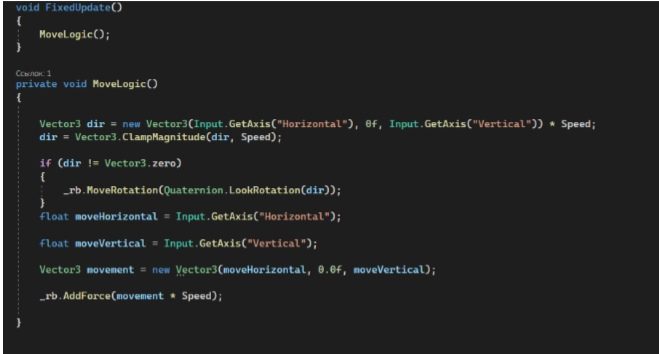
\includegraphics[width=0.8\linewidth]{forExample.jpg}

\caption{Скрипт, отвечающий за передвижение}

\label{fig:mpr}
\end{figure}
Дальше отчет идет в том же стиле
\newpage